%----------------------------------------------------------
%\usepackage{mathtext}
\usepackage{amsfonts}
%\usepackage{amsmath}
%\usepackage{mathabx}
\usepackage{MnSymbol}
\usepackage{ccicons}
\usepackage{graphicx}
%----------------------------------------------------------
%\newcommand{\doclicense}{\copyright\xspace}
%\newcommand{\doclicense}{\ccLogo\ccAttribution\xspace}%\ccShareAlike
\newcommand{\doclicense}{\includegraphics[width=0.1\textwidth]{doc-spec/by.eps}\xspace}%\ccShareAlike
%
%----------------------------------------------------------
\usepackage[T2A]{fontenc}
\usepackage[utf8]{inputenc}
\usepackage[english,russian]{babel} %% это необходимо для включения переносов
\usepackage{float}
\usepackage{listings}
\usepackage{longtable}
\usepackage{rotating}
\usepackage{multirow}
\usepackage{pdflscape}
\usepackage{bm}
\usepackage{cmap} % необходимо для возможности копирования и поиска в готовом PDF
\usepackage{array}
\usepackage{multicol}

\usepackage{hyperref}
\hypersetup{colorlinks=true, linkcolor=red}
%----------------------------------------------------------
% добавление поддержки команды вывода текста на полях \marginnote
\usepackage{marginnote}
% добавление поддержки команды \color
\usepackage{xcolor}
%--------------------------------------------
% final - удаляет все всплывающие комментарии
\usepackage[author={Alexandr Sokolov},opacity=0.1]{pdfcomment}
%\usepackage[author={Alexandr Sokolov},opacity=0.1,final]{pdfcomment}
\newcommand{\messnote}[1]{\marginnote{\color[rgb]{1,0,0}\Huge\textbf{!}\pdfcomment{#1}}[-1.0cm]}

\usepackage{pdfpages}
%----------------------------------------------------------
% необходимо для работы команды \xspace (умный пробел после замены, осуществляемой некоторой командой в тексте)
\usepackage{xspace}

\usepackage{tikz}
\usetikzlibrary{tikzmark}
%\usetikzlibrary{matrix,automata,graphs}
\usetikzlibrary{arrows,positioning,trees}

%----------------------------------------------------------
% необходимо для возможности включать в имена включаемых файлов _
\usepackage[strings]{underscore}
%----------------------------------------------------------
% Произвольная нумерация списков.
\usepackage{enumerate}
%----------------------------------------------------------
\raggedbottom
%%\hfuzz=10pt
\textwidth=163mm
\textheight=220mm
\oddsidemargin=-0.5pt
\footskip=30pt
\topmargin=27pt
\headheight=12pt
\headsep=25pt
\topskip=10pt
\baselineskip=15pt
\topmargin=-4mm
%----------------------------------------------------------
% указание 
\setcounter{secnumdepth}{2}
%----------------------------------------------------------
% подлкючение пакета для подсчета объектов
\usepackage{totcount}
% регистрируем счетчик страниц
\regtotcounter{page}
%----------------------------------------------------------
% определение атрибутов сборки Git
%\usepackage[grumpy, maxdepth=6]{gitinfo2}
%\renewcommand{\gitMark}{\textcolor{gray}{[git] \textbullet{} \gitBranch\,@\,\gitAbbrevHash{} \textbullet{} \gitAuthorName (\gitAuthorIsoDate)}}
%----------------------------------------------------------
% необходимо для того, чтобы в окружениях enumerate можно было менять формат нумерации
\usepackage{enumitem}
%----------------------------------------------------------
%Необходимо для сокращения размера шрифта подписей и сокращения отступов между рисунком и подписью к нему
\usepackage[margin=5pt,font={small, singlespacing}, labelfont={small}, justification=centering, labelsep=period]{caption}
\captionsetup{belowskip=0pt}
%----------------------------------------------------------
\usepackage[numbers]{natbib}
\usepackage{bibentry}
%***natbib, bibentry***%
% Следующий код необходим для того, чтобы исправить конфликт между пакетами natbib+bibentry и стилем оформления ссылок согласно российскому ГОСТу cp1251gost705u
\ifx\undefined\selectlanguageifdefined
\def\selectlanguageifdefined#1{}\else\fi
\ifx\undefined\BibEmph
\def\BibEmph#1{\emph{#1}}\else\fi
%----------------------------------------------------------

% подключение листингов и определение языков
%\usepackage{listingsutf8}
\usepackage{listings}

\lstset
{
		extendedchars=\true, % включаем не латиницу
%		inputencoding=utf8x,
		frame=tb, % рамка сверху и снизу
		escapechar=|, % |«выпадаем» в LATEX|
		xleftmargin=0.5cm,
		xrightmargin=0.5cm,
		columns=fullflexible,
%		aboveskip=5pt,
		numbers=left,                    % where to put the line-numbers; possible values are (none, left, right)
		numbersep=4pt,                   % how far the line-numbers are from the code
		showspaces=false,
		showstringspaces=false,
		breakatwhitespace=true,         % sets if automatic breaks should only happen at whitespace
		breaklines=true,                 % sets automatic line breaking
		basicstyle=\color{black}\small\sffamily,%\ttfamily,% \sffamily
		commentstyle=\color{gray}\itshape, % шрифт для комментариев
		stringstyle=\color{orange},
%		stringstyle=\bfseries, % шрифт для строк
		numberstyle=\footnotesize\color{gray},
%		numberstyle=\ttfamily\small\color{gray}, % the style that is used for the line-numbers
		keywordstyle=\color{blue}\bfseries,
%		directivestyle=\color{red},
%		emph={int,char,double,float,unsigned,bool,string},
		emphstyle={\color{blue}\bfseries},
		tabsize=2,
%		morecomment=[l]{//},
%		otherkeywords={=,==,:,&},
		texcl=true,
}

\lstloadlanguages{Python, C++}
%--------------------------------------------
% необходимо для команды \cancelto{0}{x}
\usepackage{cancel}
%----------------------------------------------------------
% необходимо для того, чтобы доопределить спецификатор P, для 
% использования в таблицах при форматировании
\usepackage{array}
\newcolumntype{P}[1]{>{\centering\arraybackslash}p{#1}}
%----------------------------------------%
% необходимо для того, чтобы допускались разрывы страниц внутри align align*
\allowdisplaybreaks
%----------------------------------------%
%\def\pbs{\raggedright\baselineskip3.0ex}
\def\signhrule{\raggedright\baselineskip30.0ex \vrule height 0.5pt width30mm depth0pt}

\makeatletter
\def\dynscriptsize{\check@mathfonts\fontsize{\sf@size}{\z@}\selectfont}
\makeatother
\def\textunderset#1#2{\leavevmode
  \vtop{\offinterlineskip\halign{%
    \hfil##\hfil\cr\strut#2\cr\noalign{\kern-.3ex}
    \hidewidth\dynscriptsize\strut#1\hidewidth\cr}}}

\newcommand\executer[1]{\textunderset{\scriptsize{подпись, дата}}{\signvrule} #1}
%----------------------------------------------------------
% необходимо для поддержки поворотов текста
\usepackage[absolute]{textpos}
\setlength{\TPHorizModule}{30mm}
\setlength{\TPVertModule}{\TPHorizModule}
\textblockorigin{0mm}{25mm} % start everything near the top-left corner
%----------------------------------------%
% Определение отступа от номера в подсекции
\usepackage{tocloft}
\renewcommand\cftsubsecnumwidth{2.5cm}
%----------------------------------------------------------
% Определение заголовка заметки
\newcommand{\notestatement}[2]{%
%\subsection*{\notedate: #2 (\currentauthor)}\label{#1}
\subsection*{\notedate: #2}\label{#1}
\addcontentsline{toc}{subsection}{\notedate:\hspace{10pt} #2}
}

% \pdfnotestatement{@label@}{@title@}{@pdffile@}
\newcommand{\pdfnotestatement}[3]{%
\subsection*{\notedate: #2}\label{#1}
\addcontentsline{toc}{subsection}{\notedate:\hspace{10pt} #2}
{\catcode`\_=11
\includepdf[pages=-]{#3}}
}
%----------------------------------------------------------
% оформление "теорем"
\usepackage{amsthm}
%----------------------------------------------------------
\newtheoremstyle{theoremstyle}% <name>
{0pt}% <Space above>
{0pt}% <Space below>
{\normalfont}% <Body font>
{0pt}% <Indent amount>
{\bfseries}% <Theorem head font>
{.}% <Punctuation after theorem head>
{.5em}% <Space after theorem headi>
{}% <Theorem head spec (can be left empty, meaning `normal')>
%----------------------------------------------------------
\theoremstyle{theoremstyle}
%----------------------------------------------------------
\newtheorem{question}{Вопрос}
\newtheorem{task}{Задача}
\newtheorem{solution}{Решение}
\newtheorem{remark}{Замечание}
%--------------------------------------------------
% атрибуты задачи
\newcommand{\noteattributes}[1]{%
\def\tempempty{}
\def\tempa{#1}
  \ifx\tempempty\tempa \def\tempa{\currentauthor, \notedate}\fi

\vspace{0.5cm}
\begin{flushright}
		\begin{tabular}{p{0.2\textwidth}p{0.45\textwidth}}
		\hfill Подготовлено: & \textit{\tempa} \\ %\doclicense~
		\end{tabular}
\end{flushright}
}
%----------------------------------------%
\makeatletter
\newcommand{\rndfielddscr}[1]{%
%\csname #1\endcsname (\expandafter\@gobble\string#1)} % Следует выбрать среди одного из доступных направлений
\expandafter\csname #1\endcsname\xspace (#1)}
\makeatother
%----------------------------------------%
\makeatletter
\newcommand{\rndprojectdscr}[1]{%
\expandafter\csname #1\endcsname\xspace}
\makeatother
%----------------------------------------------------------
% общие определения
\newcommand{\UpperFullOrganisationName}{Министерство науки и высшего образования Российской Федерации}
\newcommand{\ShortOrganisationName}{МГТУ~им.~Н.Э.~Баумана}
\newcommand{\FullOrganisationName}{федеральное государственное бюджетное образовательное учреждение высшего профессионального образования\newline <<Московский государственный технический университет имени Н.Э.~Баумана (национальный исследовательский университет)>> (\ShortOrganisationName)}
\newcommand{\OrganisationAddress}{105005, Россия, Москва, ул.~2-ая Бауманская, д.~5, стр.~1}
%----------------------------------------------------------
\newcommand{\TargetAudience}{%
Документ разработан для оценки результативности проведения научных исследований по направлению <<\expandafter\csname\rndfield\endcsname>>\xspace в рамках реализации курсовых работ, курсовых проектов, выпускных квалификационных работ бакалавров и магистров, а также диссертационных исследований аспирантов кафедры <<Системы автоматизированного проектирования>> (РК6) МГТУ~им.~Н.Э.~Баумана.}

\newcommand{\PrefaceIntro}{%
Документ содержит краткие материалы, формируемые обучающимися и исследователями в процессе их работ по одному научному направлению.}

\newcommand{\DocOutReference}{\textbf{\AllAuthors}. \textbf{\rndfielddscr{\rndfield}}: \DocumentType.~/ Под редакцией Соколова~А.П. [Электронный ресурс] --- \City: \Year. --- \total{page} с. URL:~\url{https://arch.rk6.bmstu.ru} (облачный сервис кафедры РК6)}

\newcommand{\Preface}{\PrefaceIntro \TargetAudience \newline \DocOutReference}
%----------------------------------------------------------
\newcommand{\DocumentType}{Научно-исследовательские заметки} % тип документа
\newcommand{\SubTitle}{по направлению <<\rndfielddscr{\rndfield}>>}
%----------------------------------------------------------
